\documentclass[11pt,letterpaper]{article}
\usepackage[utf8]{inputenc}
\usepackage[left=1in,right=1in,top=1in,bottom=1in]{geometry}
\usepackage{amsfonts,amsmath,dsfont}
\usepackage{graphicx}
% -----------------------------------
\usepackage{hyperref}
\hypersetup{%
  colorlinks=true,
  linkcolor=blue,
  citecolor=blue,
  urlcolor=blue,
  linkbordercolor={0 0 1}}
% -----------------------------------
\usepackage[authordate,backend=biber]{biblatex-chicago}
\addbibresource{citation.bib}
% -----------------------------------
\title{Plotting and Fitting Power-Laws}
\author{Ryan Sh\`iji\'e D\`u}
\date{\today}
% -----------------------------------
% \setlength{\parindent}{0.0in}
\setlength{\parskip}{0.1in}
% -----------------------------------
\begin{document}
\newcommand{\de}{\mathrm{d}}
\newcommand{\DD}{\mathrm{D}}
\newcommand{\pe}{\partial}
\newcommand{\mcal}{\mathcal}
%\newcommand{\pdx}{\left|\frac{\partial}{\partial_x}\right|}

\newcommand{\dsp}{\displaystyle}

\newcommand{\norm}[1]{\left\Vert #1 \right\Vert}
%\newcommand{\mean}[1]{\left\langle #1 \right\rangle}
\newcommand{\mean}[1]{\overline{#1}}
\newcommand{\inner}[2]{\left\langle #1,#2\right\rangle}

\newcommand{\ve}[1]{\boldsymbol{#1}}

\newcommand{\thus}{\Rightarrow \quad }
\newcommand{\fff}{\iff\quad}
\newcommand{\qdt}[1]{\quad \mbox{#1} \quad}

\renewcommand{\Re}{\mathrm{Re}}
\renewcommand{\Im}{\mathrm{Im}}
\newcommand{\E}{\mathbb{E}}
\newcommand{\lap} {\nabla^2}
\renewcommand{\div}{\nabla\cdot}

\newcommand{\hot}{\text{h.o.t.}}

\newcommand{\ssp}{\left.\qquad\right.}

\newcommand{\var}{\text{var}}
\newcommand{\cov}{\text{cov}}

\newcommand{\csch}{\text{csch}}
\newcommand{\sech}{\text{sech}}

\newcommand{\MATLAB}{\textsc{Matlab}}




% -----------------------------------
\maketitle

\section{Introduction}
In applied math, data often follow power-laws of the form:
\begin{align}
    y(x) = Cx^\gamma.
\end{align}
Here $\gamma$ is the power-law exponent. For example, in turbulence theory, conserved quantities often distribute over scales (wave-numbers $k$) following a power-law. One result of this kind is the famed ``Kolmogorov $5/3$ law'' which states that the kinetic energy spectrum $E(k)$ of 3D hydrodynamics turbulence follows the law \parencite{Frisch_95}:
\begin{align}
    E(k) = Ck^{-5/3}.
\end{align}
Another example is in the field of numerical analysis. Numerical integration schemes commonly have errors asymptotically proportional to powers of discretization step size. To give two concrete cases: 1. composite trapezoidal rule for integration has error asymptotically following
\begin{align}
    e(h) = Ch^{2}
\end{align}
and 2. explicit Runge–Kutta 4\textsuperscript{th} order method (Rk4) for solving differential equations has
\begin{align}
    e(h) = Ch^{4}
\end{align}
where $h$ is (spatial or temporal) discretization step size \parencite{SuliMayers_03}. It suffices to say there are more examples than the ones listed, and power-laws are constantly being plotted and analyzed.

Power-laws are commonly visualized using a log-log plot, where the $x$ and $y$-axis are in log scale and power-laws appear as straight lines. To obtain the power-law exponent, it is common to use linear regression on the log-log scale data. In \S\ref{sec_linreg_log} this note we will examine the application of linear regression on data distributed following power-laws and conclude that while it is appropriate in many cases, the choice of cost function deserves more case-specific consideration. \S\ref{sec_plot_log} gives our suggestions for plotting data following power-laws. This necessitates a discussion of when it is appropriate to diagnose a power-law exponent from data.

\section{Diagnosing power-law exponent from data}\label{sec_linreg_log}
We will work with the general power-law
\begin{align}
    y(x) = Cx^\gamma.\label{eq_gen_pl}
\end{align}
We assume that the data $z$ follows \eqref{eq_gen_pl} with small deviations: 
\begin{align}
    z(x) = Cx^\gamma + \epsilon.\label{eq_data_pl}
\end{align}
Assumptions on the form of the error and how we measure it will dictate the best regression to use. Only in some cases is the common linear regression on the log-log scale appropriate. 
% For notational convenience, we name $\alpha:= \log x$ and $\beta:= \log z$.

\subsection{Scaled $L^2$ norm}\label{sec_scale_L2}
One interpretation of regression with least square error is that it is the orthogonal projection onto the selected basis functions. The projection minimizes the functional $L^2$ norm:
\begin{align}
    \int \left| \log z- (\log C+\gamma \log x) \right|^2 \de(\log x).\label{eq_log_L2}
\end{align}
We focus on
\begin{align}
    \log z- (\log C+\gamma \log x) &= \log z- \log y = \log z- \log (z-\epsilon).
\end{align}
We assume that the deviation $\epsilon$ is small so that Taylor expansion is appropriate. We have
\begin{align}
    &\log z- \log (z-\epsilon) \approx \frac{\epsilon}{z}\\
    \thus &\log z- (\log C+\gamma \log x) \approx \frac{z-Cx^\gamma}{z}.
\end{align}
We replace the integrand in \eqref{eq_log_L2} 
\begin{align}
    \int \left|\frac{z-Cx^\gamma}{z}\right|^2 \de(\log x).
\end{align}
A change of variable to $\de x$ gives
\begin{align}
    \int \left|\frac{z-Cx^\gamma}{z}\right|^2 \frac{1}{x} \;\de x.\label{eq_L2_scale1/x}
\end{align}
Without the $1/x$ factor, we see that linear regression on the log-log scale is in fact minimizing the $L^2$ error relative to the values of the data $z$. This normalization is desirable in some cases: because the data follow power-laws, their magnitude can change significantly over a large range of $x$. If the error scale as the magnitude of the data, it is appropriate to minimize the relative error. However, if we know \textit{a priori} the error magnitude is uniform, the normalized error is not appropriate.

\subsection{Density of data}
The $1/x$ factor comes from the change of variable in the integration. We will show that it directly relates to the density of the discrete data. We have focused on the integral functional norm, but we only have discrete data. One way to relate them is to use the discrete data to numerically approximate the integration. A factor will appear if the data are distributed unevenly. Take the example of turbulence spectra, we have data for each integer wavenumber $x$. This means in the log-log scale, the data appear at each $\log x$ and have gaps of approximate size $1/x$. The simple sum error used in linear regression on the log-log scale
\begin{align}
    \sum_i \left| \log z_i- (\log C+\gamma \log x_i) \right|^2\label{eq_err_simple_sum}
\end{align}
is a discrete approximation of the scaled integral
\begin{align}
    \int x \left| \log z- (\log C+\gamma \log x) \right|^2 \de(\log x).
\end{align}
Intuitively, the $x$ factor is due to the denser data for larger $x$. Apply the calculations in \S\ref{sec_scale_L2} we have that it is approximately equivalent to
\begin{align}
    \int \left|\frac{z-Cx^\gamma}{z}\right|^2 \;\de x\label{eq_reg_rel_L2}
\end{align}
the integrated relative error squared. Because the data are distributed evenly in $x$, the $1/x$ factor disappears in integration with regards to $x$. \eqref{eq_err_simple_sum} and \eqref{eq_reg_rel_L2} connect the commonly used linear regression on the log-log scale to a more interpretable relative $L^2$ error on the unscaled data. For diagnosing the power law exponent of turbulence spectra, this interpretation is the most appropriate. This is the interpretation assumed in \cite{DuBuhler_23} when they diagnose power laws for turbulence spectra.

In other cases, the data is collected with an even distance in $\log x$. For example, to check the convergence of a numerical scheme, one usually uses results with discretization step $h, h/2, h/4, \dots$. In these situations, the simple sum \eqref{eq_err_simple_sum} is an approximation of \eqref{eq_L2_scale1/x}. The $1/x$ appears because the data distribute unevenly in $x$. 

\subsection{Maximum likelihood interpretation}
An alternative interpretation of inference using least square error is that it maximizes the log-likelihood function assuming the deviations are independent and Gaussian. Further assuming that the errors have uniform standard deviations in the log-log scale, we recover the error \eqref{eq_err_simple_sum}. To retain the Gaussian nature of the errors, we assume again that the error is small so that the linear Taylor expansion is a sufficient approximation. Then for $x$ and $z$, this means the errors are independent Gaussians with standard deviations that scale as $z$. We have the cost function
\begin{align}
    \sum_i \left|\frac{z_i-Cx_i^\gamma}{z_i}\right|^2.
\end{align}
This is the underlying interpretation for the regression in Figure 3 of \cite{DuBuhler_23}.

Alternatively, assuming that the error is uniform in the regular scale, maximum likelihood minimizes
\begin{align}
    \sum_i \left|z_i-Cx_i^\gamma\right|^2 \iff \sum_i \left| z_i\left(\log z_i- (\log C+\gamma \log x_i)\right) \right|^2.\label{eq_iff_sum_KL}
\end{align}
We see that the maximum likelihood interpretation recovers the result of the functional $L^2$ norm interpretation except the scaling due to data density. Indeed, with the assumption of independence, the maximum likelihood interpretation takes no account of the distribution of data in $x$.

\subsection{$\ell^1$ norm and KL divergence}
We pay special attention to the right-hand-side equation in \eqref{eq_iff_sum_KL}. Instead of the squared sum, we sum the absolute values ($\ell^1$ norm). We have
\begin{align*}
    \sum_i \left| z_i\left(\log z_i- \log y_i\right) \right| &= \sum_i \left| z_i \log\left( \frac{z_i}{y_i}  \right) \right| = D\textsubscript{KL}[z||y]
\end{align*}
where $D\textsubscript{KL}$ denotes the Kullback–Leibler (KL) divergence. Note the KL divergence is not a norm. The loss of symmetry between $y$ and $z$ comes from the choice of $z$ as the center for the Taylor expansion. We could understand this surprising connection by noting that many probability distributions of interests have power-law tails (e.g.: Cauchy distribution). This opens the tools of applying the tools of probability and information theory to our problem.

\section{Plotting data following power-laws}\label{sec_plot_log}
We have addressed how to diagnose the power-law exponent from data. However, it is not always appropriate to do the diagnostic in the first place. In many cases, we know the power-law exponent the data should follow. Then we should plot the data and the theoretical power-law on the same plot and compare them, instead of fitting a power-law to the data. We will showcase this point using some examples. They will also serve as examples of plotting data that follows power-laws.

\subsection{Turbulence spectra}
Data measuring turbulence spectra are commonly plotted on the log-log scale. We often know the power-law it should follow from theory. Figure \ref{fig_turb_spec_eg} is an example of such a plot, and it does several things right. Since we know the power-law, we should not measure the exponent from data. Instead, this figure plots the power-law alongside the data and we can compare the data and theory easily. Additionally, this plot labels its axes correctly. It is more stylistic to label the axes using raw values, instead of labeling them using $\log x$ and $\log y$ and the correspondent $\log$ values. And it is \textit{incorrect} to label the numbers using the unscaled numbers ($10^1, 10^2, \dots$), and label the axes $\log x$ and $\log y$. That would mean $\log x = 10^1, 10^2, \dots$ and is absurd. In \MATLAB, the numerical labels are automatically correct, and one only have to make sure that the text labels are not in $\log$. Finally, since we have discrete data, it is better to plot the data as discrete data points and not connect them.
\begin{figure}
    \centering
    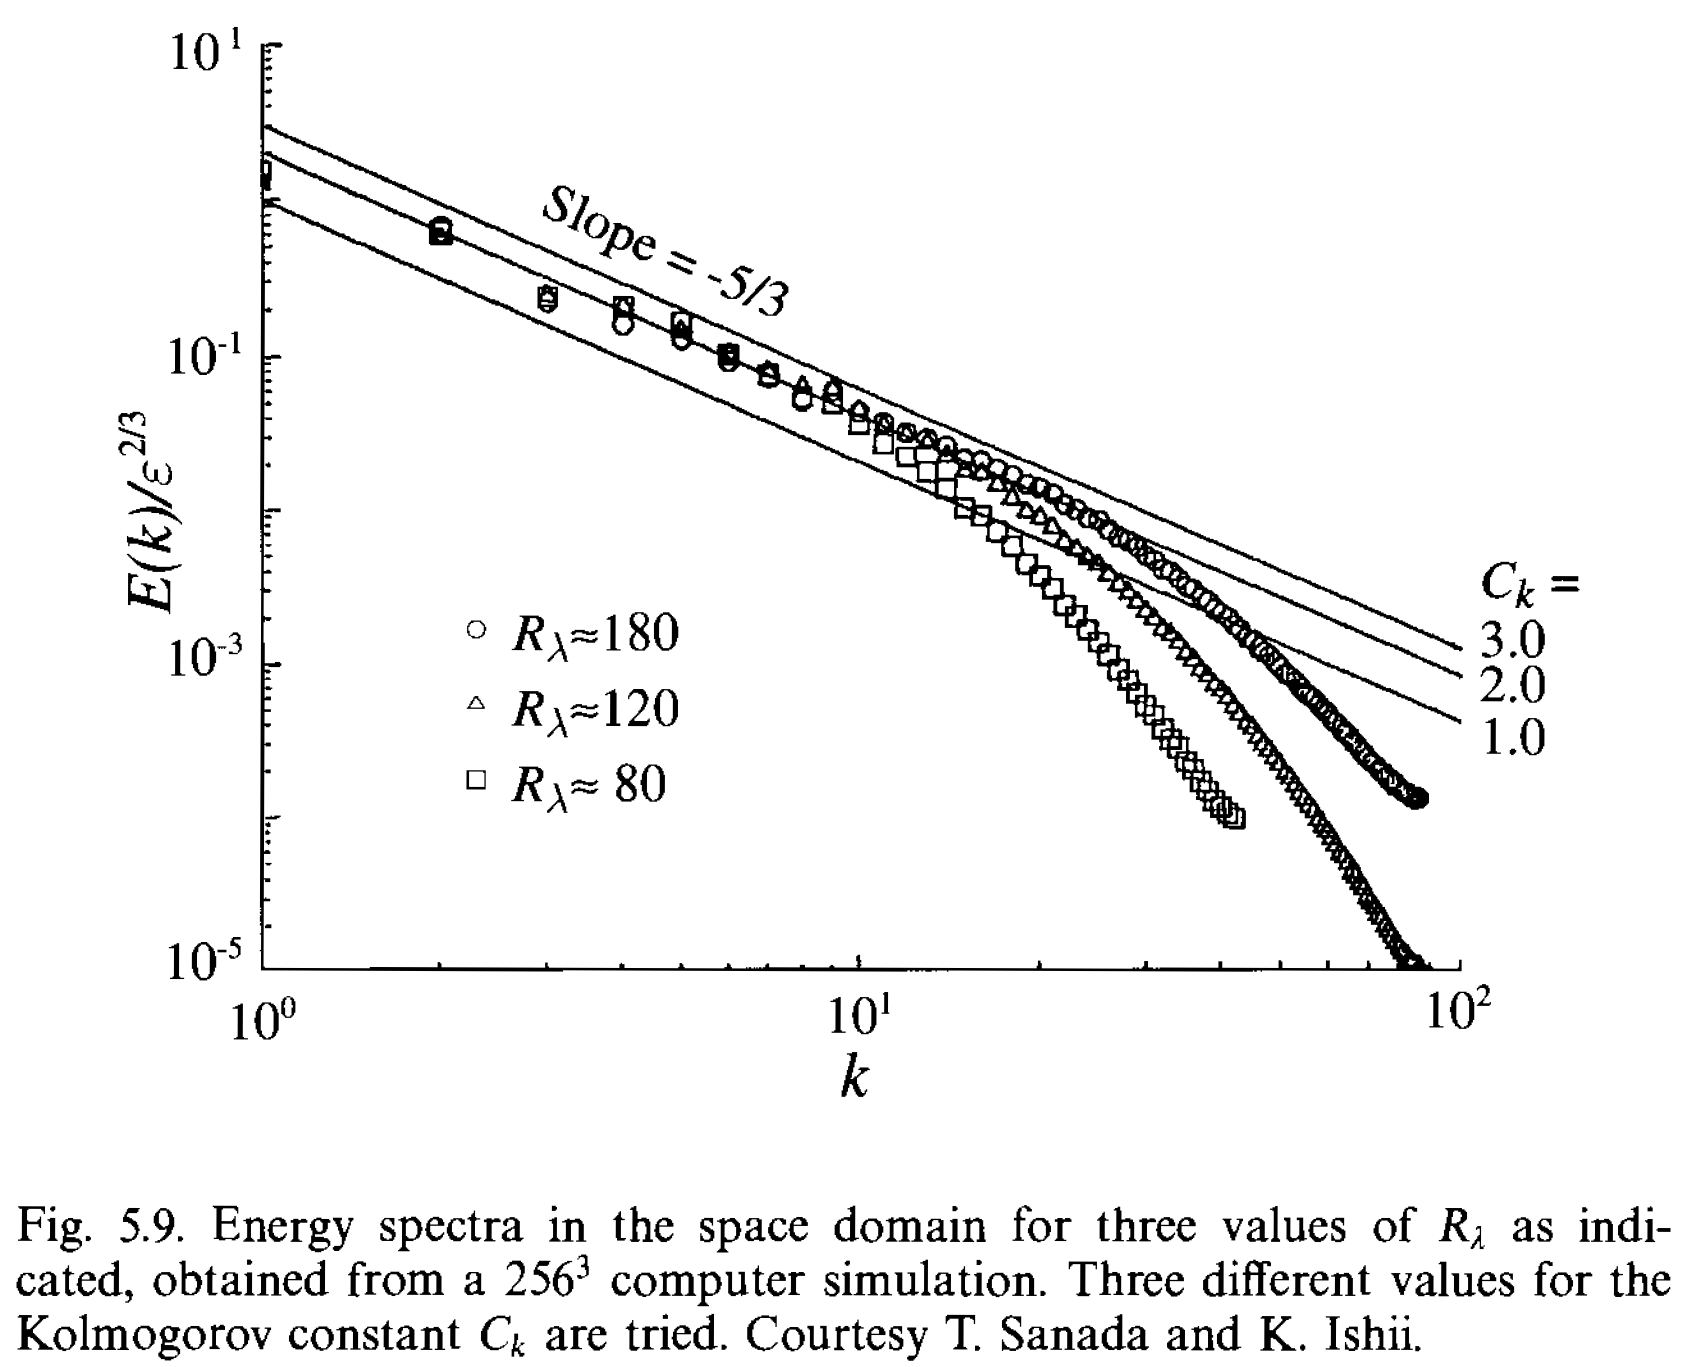
\includegraphics[width = 0.6\textwidth]{figs/turb_spec_eg}
    \caption{Example plot from \cite[Fig. 5.9.]{Frisch_95}.}
    \label{fig_turb_spec_eg}
\end{figure}

\subsection{Numerical errors}
The same principle applies to plotting numerical errors. Figure \ref{fig_numInt_example} shows an example of a clear plot. The axes are labeled correctly. Power-laws are not diagnosed, instead, the theoretical power-law is plotted alongside the data so that their agreements and differences are clear at one glance. The data are plotted using dots to signify their discreteness.
\begin{figure}
    \centering
    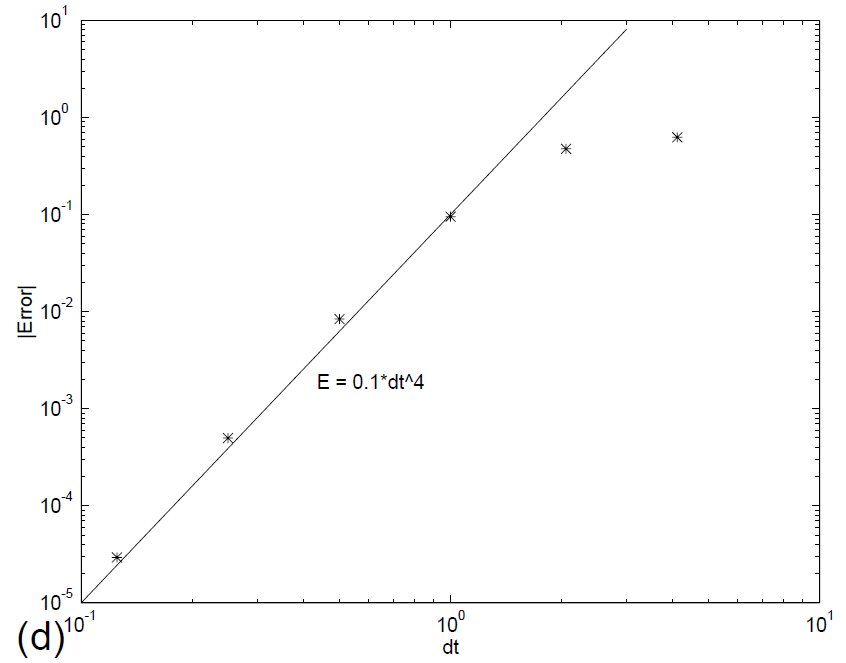
\includegraphics[width = 0.6\textwidth]{figs/numInt_example}
    \caption{Example plot from Figure 1d of \cite{MilewskiTabak_99}. Original label: {\small Propagation of an oblique solitary wave, with parameters $\epsilon = 0.1$ and $k = \frac{1}{\sqrt{5}}(2,1)$, in a grid with periods $L = 14\pi$ and $H = 28\pi$ and $256 \times 256$ points. (d) Log-log plot of the normalized error after one tour of the periodic box, as a function of $\Delta t$.}}
    \label{fig_numInt_example}
\end{figure}

\section{Concluding remarks}
This note treats the topics of when and how to diagnose power-law exponents from data. We conclude that not all situations require the diagnostics of power-law exponents via regression. And in situations when their diagnostics are appropriate, there are subtleties in choosing the correct cost functions to minimize for regression. One must take care when plotting and analyzing data that follow power-laws.

\section*{Acknowledgment}
We were inspired to think more about fitting power-law while working with  Oliver B\"uhler on \cite{DuBuhler_23}. We thank him for pointing out that relative error is sometimes the appropriate measure of error. We learned many lessons on plotting from Aleksandar Donev, some of them are included in this note. We thank him for teaching us to think carefully before we plot. 


\newpage
\printbibliography

\end{document}
